\mychapter{Nombres reals}{Nombres reals}{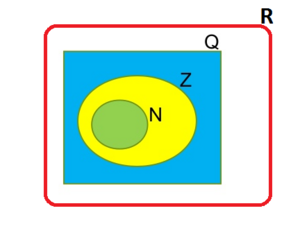
\includegraphics[width=4cm]{img-01/chap1.png}}
{chap:real}
 
\section{La recta real}

\begin{tip}
	Els nombres reals es classifiquen en: Naturals $\mathbb{N}=\{1,2,3,\cdots \}$, \par Enters $\mathbb{Z}=\{\cdots,-2,-1, 0, 1,2,\cdots \}$, Racionals $\mathbb{Q}=\{\frac{a}{b},\, a $ i $ b\neq 0 $ enters $  \}$, \par Irracionals $\mathbb{I}=\{\sqrt{2}, \pi, e, \cdots \}$ i els nombres reals  $\mathbb{R}=\mathbb{Q}\cup \mathbb{I}$.\par
		\rule{\textwidth}{1pt}
		
	El \textbf{valor absolut} d'un nombre és $|a|=a$ si $a\geq 0$, $|a|=-a$ si $a<0$.
	
	La \textbf{distància} entre dos nombres es troba mitjançant $\mathrm{Dist}(a,b)=|b-a|$. 

\end{tip}

\begin{mylist}
  
	\exer \spen
		 Troba l'expressió decimal de les fraccions
		\begin{tasks}(3)
			\task $\dfrac{2}{3}=$
			\task $\dfrac{3}{4}=$
			\task $\dfrac{7}{30}=$
			\task $\dfrac{6}{25}=$
			\task $\dfrac{7}{8}=$
			\task $\dfrac{9}{11}=$	
		\end{tasks} 
	\answers{[$0.\hat 6$, $0.75$, $0.2\hat 3$, $0.24$, $0.875$, $0.\widehat{81}$]}

	\exer  Escriu en forma de fracció les següents expressions decimals periòdiques, redueix-les i comprova que està bé:
	\begin{tasks}(4)
		\task $2,353535{\cdots}$
		\task $87,23656565{\cdots}$
		\task $0,9999{\cdots}$
		\task $26,5735735735{\cdots}$
	\end{tasks} 
\answers{[$233/99$, $431821/3300$, $1$]}
  	
    \pagebreak
	\exer  Representa a la recta numèrica els següents nombres racionals:
	\begin{tasks}(4)
		\task $\dfrac{9}{5} $
		\task $\dfrac{-13}{4} $
		\task 1,342
		\task $-$2,555555{\dots}
	\end{tasks} 


	\exer  Representa a la recta numèrica els nombres irracionals:
	\begin{tasks}(4)
		\task $\sqrt{10} $
		\task  $-\sqrt{6} $
		\task $\sqrt{27} $
		\task 	$\dfrac{1+\sqrt{5} }{2} $ 
	\end{tasks}
 
	\exer \spen Escriu el valor absolut dels següents nombres: 
	\begin{tasks}(3)
		\task $|5|=$
		\task $|-5|=$
		\task $|\pi-\sqrt{10}|=$
	\end{tasks}
\answers[cols=3]{[5, 5, $\sqrt{10}-\pi$]}
 

	\exer  Representa a la recta real i calcula la distància entre els nombres reals següents: 
	\begin{tasks}(2)
		\task Dist(5 , 9) 
		\task Dist($-$2.3 , $-$4.5)
		\task Dist($-$1/5 , 9/5)
		\task Dist($-$3.272727{\dots}. ,  6.27272727{\dots}.)
	\end{tasks}
\answers{[4, 2.2, 2, 9]}
  
	
\section{Intervals i entorns}
	
	\exer  Escriu els següents intervals mitjançant conjunts i representa'ls a la recta real:
	\begin{tasks}(4)
		\task $[1, 7)$ 
		\task $(-3, 5)$
		\task $(2, 8]$ 
		\task ($-\infty$, 6)
	\end{tasks}
\answers{[$1\leq x<7$, $-3<x<5$, $2<x\leq8$, $x<6$]}
 


	\exer  Representa a la recta real i escriu en forma d'interval:
	\begin{tasks}(4)
		\task  $2 < x < 5$
		\task  $4 < x$
		\task $3 \leq x < 6$
		\task 	$x \leq 7$
	\end{tasks}
\answers{[$(2,5)$, $(4,+\infty)$, $[3,6)$, $(-\infty,7]$]}

 

	\exer \spen Expressa com a interval o semirecta, en forma de conjunt (emprant desigualtats) i representa'ls gràficament:
	
	   \begin{tasks}
	   	\task  Un percentatge superior al 26 \% \dotfill
		%
		\task  Edat inferior o igual a 18 anys \dotfill
		%
		\task  Nombres, el cub dels quals, sigui superior a 8 \dotfill
		%
		\task  Nombres positius la part entera dels quals té 3 xifres \dotfill
		%
		\task  Temperatura inferior a 25 ºC \dotfill
		%
		\task  Nombres pels quals existeix la seva arrel quadrada  \dotfill
		%
		\task  Nombres que estiguin de 5 a una distància inferior a 4 \dotfill
	\end{tasks}
\answers{[$(26,100]$, $[0,18]$, $(2,+\infty)$, $[100,1000)$, $(-\infty,25)$, $[0,+\infty)$, $(1,9)$]}

\end{mylist}
\begin{theorybox}[Entorn obert]
	Es defineix l'entorn obert de centre $a$ i radi $r$, i s'escriu $E(a,\, r)$, com l'interval $(a-r, a+r)$ 
\end{theorybox}

\begin{resolt}{
	Expressa l'interval $(-1,5)$ com un entorn. }
	
	El centre es troba al punt mitjà $a=2$ i el radi és $r=3$, és a dir $(-1,5)=E(2,\, 3)$
\end{resolt}

 
\begin{mylist}
 
	\exer  Expressa en forma d'interval els següents entorns:
	\begin{tasks}(3)
		\task \textit{E}(1, 5)
		\task \textit{E}($-2$, $\frac{8}{3} $ )
		\task \textit{E}($-10$, $0.001$)
	\end{tasks}
\answers{[$(-4,6)$, $(-14/3,2/3)$, $(-10.001,-9.999)$]}
 
 
	\exer  Expressa en forma d'entorn els següents intervals:
	\begin{tasks}(3)
		\task $(4,\, 7)$
		\task $(-7,\, -4)$
		\task $(-3,\, 2)$
	\end{tasks}
\answers{[$(5.5,1.5)$, $(-5.5,1.5)$, $(-0.5,2.5)$]}
 

\exer Calcula $x$ en les següents equacions: (pista: $x$ pot tenir dos valors)
\begin{tasks}(3)
	\task $|x|=5$
	\task $|x-4|=0$
	\task $|3x+9|=21$
\end{tasks}
\answers{[$x=$ 5 i --5, $x=$ 4, $x=$ --10 i 4]}
 


\exer Representa a la recta real els nombres que verifiquen les següents relacions:
\begin{tasks}(4)
	\task $|x|<1$
	\task $|x|\leq 1$
	\task $|x-3|>1$
	\task $|x-3|\geq 1$
\end{tasks}
\answers[cols=1]{[$(-1,1)$, $(-\infty,-1]\cup [1,+\infty]$, $(-\infty,2)\cup(4,+\infty)$, $(-\infty,2]\cup[4,+\infty)$]}


\exer Troba dos nombres que distin 6 unitats de 3, i altres dos que distin 3,5 unitats de $-$2, calcula després la diferència entre el major i el menor de tots aquests nombres. 
\answers{$-3$ i $9$. $-5.5$ i $1.5$. $9-(-5.5)=14.5$}

\exer Escriu l'interval [$-$3, 5] $\mathrm{\cap}$ (3, 8).
\answers{$[-3, 8)$}
 
\exer Escriu l'interval format pels nombres reals x que compleixen $|x-8|\leq 3$. 
\answers{$[5,11]$}

\exer Determina els conjunts A $\mathrm{\cap}$  B, A  $\cup$ B, A $-$ B i $-$A en els casos següents:
\begin{tasks}(2)
	\task A = [\textit{$-$}11, \textit{$-$}9]; B = (\textit{$-$}1, 6)
	\task  A = [\textit{$-$}5, 5]; B = (3, 4)	
\end{tasks}
 \answers{[$A\cap B=\emptyset$;\par $A\cup B=[-11,-9] \cup (-1,6)$;\par $A-B=A$,  
 		   $A\cap B=B$; $A\cup B=A$;\par $A-B=[-5,3]\cup [4,5]$]}
 
\end{mylist}
 

\section{Radicals}

\begin{theorybox}
	Trobareu un resum de les propietats dels radicals a la pàgina \pageref{page:pradicals}.
\end{theorybox}

\begin{mylist}
	
\exer[1]  Expressa com un sol radical:
\begin{tasks}(3)
\task $\sqrt{\sqrt[{3}]{5} } =$          
\task $\sqrt[{4}]{\sqrt[{}]{8} } $=                   
\task $\sqrt{\sqrt{x^{3} \sqrt{x} } } $=
\end{tasks}
\answers[cols=3]{[$\sqrt[{6}]{5} $,  $\sqrt[{8}]{8} $,  $\sqrt[{8}]{x^{7} } $]}

\exer[1] Simplifica, extraient tots els factors que puguis del radical:
\begin{tasks}(4)
	\task  $\sqrt[{4}]{64} $=      
	\task  $\sqrt[{}]{243} $=          
	\task  $\sqrt[{9}]{216} $=      
	\task  $\sqrt[{8}]{1024} $=
	\task  $\sqrt[{15}]{243} $=   
	\task  $\sqrt[{6}]{2401} $= 
	\task  $\sqrt[{16}]{49} $=      
	\task  $\sqrt[{14}]{128} $=
\end{tasks}
\answers{[$2\,\sqrt[{}]{2} $,   $9\,\sqrt[{}]{3} $,     $\sqrt[{3}]{6} $,    $2\,\sqrt[{4}]{2} $,  $\sqrt[{3}]{3} $,     $\sqrt[{3}]{49} $,       $\sqrt[{8}]{7} $,   $\sqrt{2} $]}

\exer[1] Redueix el radical a l'\'{i}ndex indicat:
\begin{tasks}(4)
	\task $\sqrt[{4}]{2^{3} } =\sqrt[{12}]{2^{\_ \_ } } $    
	\task $\sqrt{7} =\sqrt[{16}]{7^{\_ \_ } } $    
	\task $\sqrt[{4}]{a^{6} } =\sqrt{a^{\_ \_ } } $     
	\task $\sqrt[{6}]{5^{12} } =\sqrt[{3}]{5^{\_ \_ \_ } } $
\end{tasks}
\answers{[$\sqrt[{4}]{2^{3} } =\sqrt[{12}]{2^{9} } $,       $\sqrt{7} =\sqrt[{16}]{7^{8} } $,    $\sqrt[{4}]{a^{6} } =\sqrt{a^{3} } $,     $\sqrt[{6}]{5^{12} } =\sqrt[{3}]{5^{6} } =5^{2} $]}

\exer[1] Expressa com un sol radical (redueix, primer de tot, els radicals a \'{i}ndex com\'{u} i simplifica si pots):  
\begin{tasks}(2)
	\task $\dfrac{\sqrt[{6}]{32} \, \cdot \, \sqrt[{3}]{25} \, }{\sqrt{8} } $   
	\task $\dfrac{\sqrt{2} \, \cdot \, \sqrt[{3}]{3} }{\sqrt[{4}]{6} } $   
	\task $\dfrac{\sqrt{5} \, \cdot \, \sqrt[{3}]{5} }{\sqrt[{4}]{5} } $     
	\task $\sqrt{\sqrt{\sqrt{2^{24} } } } $
	\task $\left(\sqrt[{5}]{64} \right)^{4} $   
	\task $\sqrt[{3}]{\sqrt{\sqrt[{3}]{5^{9} } } } $   
	\task $\sqrt{3\, \sqrt{3\, \sqrt{3^{2} } } } $    
	\task $\left(\sqrt{\sqrt[{3}]{125} } \right)^{4} $
\end{tasks}
\answers[cols=2]{[$\sqrt[{3}]{5/4} $,      $\sqrt[{12}]{2^{3} \cdot 3} $,  $\sqrt[{12}]{5^{7} } $,   $2^{3} $,      $2^{4} \cdot \sqrt[{5}]{2^{4} } $,     $\sqrt[{}]{5} $,      3,       $5^{2} $]}

\begin{example}
	a) $\dfrac{\sqrt[{6}]{32} \, \cdot \, \sqrt[{3}]{25} \, }{\sqrt{8} } =     \dfrac{\sqrt[{6}]{32} \, \cdot \, \sqrt[{6}]{25^2} \, }{\sqrt[6]{8^3} } =
	\sqrt[6]{\dfrac{2^5 \, \cdot \, 5^4 \, }{2^9 }} = \sqrt[6]{\dfrac{  5^4 \, }{2^4 }} =\sqrt[3]{\left(\dfrac{  5 }{2 }\right)^2 }
	$ 
\end{example}

\exer[1] Calcula, extraient primer factors fora dels radicals:
\begin{tasks}(2)
	\task $\sqrt{1331} $ - $\sqrt{44} $ + 2 $\sqrt{99} $=  
	\task $\sqrt[{3}]{16} $ + $\sqrt[{3}]{686} $ - 3 $\sqrt[{3}]{2} $= 
	\task 2 $\sqrt{54} $ - $\sqrt{216} $ - $\sqrt{\frac{6}{25} } $= 
	\task $\sqrt[{4}]{32} $ + $\sqrt[{4}]{\frac{2}{81} } $ - 7 $\sqrt[{4}]{2} $=
	\task 2 $\sqrt{3} $ - $\frac{1}{5} $ $\sqrt{27} $ + $\frac{2}{3} $ $\sqrt{12} $= 
	\task $\sqrt{32} $ - $\sqrt{18} $ + $\frac{1}{5} $ $\sqrt{128} $=
\end{tasks}
\answers{[
		$15\,\sqrt[{}]{11} $,  $6\,\sqrt[{3}]{2} $,      $-\sqrt[{}]{6} /5$,    $-14\,\sqrt[{4}]{2} /3$,    $41\,\sqrt[{}]{3} /15$,    $13\,\sqrt[{}]{2} /5$]}

   \begin{example}
	a) $\sqrt{1331} - \sqrt{44}  + 2 \sqrt{99} = \sqrt{11^3}  - \sqrt{2^2\cdot 11}  + 2 \sqrt{3^2 \cdot 11} =$ 
	
	\qquad\qquad\qquad\qquad\qquad\qquad = $11\sqrt{11}  - 2\sqrt{11}  + 2\cdot 3 \sqrt{11}= 15\sqrt{11}$ 
	\vspace{0.25cm} 
\end{example}

\exer[1] Desenvolupa $\left(1+\left(1+\sqrt{a} \right)^{2} \right)^{2} =$
\answers{$(2+a)^{2} +4(2+a)\sqrt{a} +4a$}

\exer[1] Racionalitza:
\begin{tasks}(3)
	\task $\dfrac{1}{\sqrt[{3}]{3} } $ =     
	\task $\dfrac{3}{2\, \sqrt[{4}]{2} } $=        
	\task $\dfrac{3}{\sqrt{2} -1} $=
	\task $\dfrac{\sqrt{2} +1}{\sqrt{2} -1} $   
	\task $\dfrac{\sqrt{2} }{\sqrt{5} +\sqrt{3} } $=    
	\task $\dfrac{2+\sqrt{5} }{2-\sqrt{5} } $=
\end{tasks}
\answers[cols=2]{[$\frac{\sqrt[{3}]{3^{2} } }{3} $, $\frac{3}{4} \,\sqrt[{4}]{2^{3} }$,  $3(\sqrt{2+1} )$,   $3+2\sqrt{2} $,    $(\sqrt{10} -\sqrt{6} )/2$,    $-(9+4\sqrt{5} )$]}

\begin{example}
	d)  $\dfrac{\sqrt{2} +1}{\sqrt{2} -1} = \dfrac{(\sqrt{2} +1)}{(\sqrt{2} -1)} \cdot \dfrac{(\sqrt{2} +1)}{(\sqrt{2} +1)} = \dfrac{(\sqrt{2} +1)^2}{(\sqrt{2})^2 -1^2}=3+2\sqrt{2}$   
\end{example}
 
\exer[1] Opera, racionalitza i simplifica
\begin{tasks}(2)
	\task $\dfrac{\sqrt{48} }{\frac{\sqrt{8} }{3} } =$  
	\task $\dfrac{\sqrt[{4}]{2} }{\frac{2}{\sqrt{2} } } =$ 
	\task $\dfrac{\frac{1}{2} }{\frac{\sqrt{3} }{3} } =$        
	\task  ${\rm (4}\sqrt{{\rm 5}} +{\rm 3}\sqrt{{\rm 5}} {\rm )}\, {\rm \cdot }\, {\rm (4}\sqrt{{\rm 5}} -{\rm 3}\sqrt{{\rm 5}} {\rm )}$=  
	\task ${\rm 2}^{-{\rm 5}} \, {\rm \cdot }\, {\rm 2}^{\frac{{\rm 1}}{{\rm 3}} } \, {\rm \cdot }\, \sqrt{{\rm 2}^{{\rm 5}} } =$
	\task $\left(\frac{{\rm 5}}{{\rm 2}} -\sqrt{{\rm 2}} \right)^{{\rm 2}} =$ 
%	\task $\dfrac{\frac{1}{2} +\frac{3}{7} }{2-\frac{4}{6} } =$    
\end{tasks}
\answers[cols=2]{[$3\sqrt{6}$,     $\frac{\sqrt[{4}]{2^{3} } }{2} $,    $\frac{\sqrt{3} }{2} $,     35,    $2^{-64/15} $,    $33/4-5\sqrt{2} $]}

\end{mylist}

\pagebreak






\begin{autoaval}{21}

\begin{mylist}
	
	\exer[2] Resol l'equació $|3x+9|=21$.
	\begin{comment}
	\begin{tasks}(4)
	\task $x=10$, $x=-4$
	\task $x=10$ 
	\task $x=-10$, $x=4$
	\task $x=-4$
	\end{tasks}
	\end{comment}
	\answers{$x=-10$ i $x=4$}		
			
	\exer[2] Expressa $\sqrt[4]{x\sqrt{x}}$ com una única arrel.
	\begin{comment}
	\begin{tasks}(4)
		\task $\sqrt[4]{x^2}$
		\task $\sqrt[8]{x^2}$
		\task $\sqrt[8]{x^3}$
		\task $\sqrt{x^{4}}$	
	\end{tasks}
	\end{comment}
	\answers{$\sqrt[8]{x^3}$}

	\exer[2] Simplifica l'expressió $(2\sqrt{3}+1)^2$.
	\begin{comment}
	\begin{tasks}(4)
	\task 7
	\task 13
	\task $7+4\sqrt{3}$
	\task $13+4\sqrt{3}$	
	\end{tasks}	
	\end{comment}
	\answers{$13+4\sqrt{3}$}
	


	\exer[2] Racionalitza l'expressió $\dfrac{4}{\sqrt{5}}$.
	\begin{comment}
\begin{tasks}(4)
\task $\dfrac{4\sqrt{5}}{5}$ 
\task $4\sqrt{5}$ 
\task $20 \sqrt{5}$ 
\task $\dfrac{20\sqrt{5}}{4}$ 
\end{tasks}	
	\end{comment}
\answers{$\dfrac{4\sqrt{5}}{5}$}


	\exer[2] Simplifica l'expressió $\sqrt[3]{54} + \frac{2}{3}\sqrt[3]{16}$.
	\begin{comment}
\begin{tasks}(4)
\task $\frac{5}{3}\sqrt[3]{70}$
\task $\frac{5}{3}\sqrt[3]{70}$
\task $\frac{13}{3}\sqrt[3]{2}$
\task $13\sqrt[3]{2/3}$	
\end{tasks}	
	\end{comment}
\answers{$\frac{13}{3}\sqrt[3]{2}$}


	\exer[2] Racionalitza l'expressió $\dfrac{2\sqrt{5}-\sqrt{3}}{\sqrt{5}+2\sqrt{3}}$.
\answers{$\dfrac{16-5\sqrt{15}}{-7}$}
 

	\exer[2] Donats els intervals $A=[-11,6]$ i $B=(-1,9)$, calcula $A\cap B$.
	\begin{comment}
\begin{tasks}(4)
\task $(-11,9)$
\task $[-11,9)$
\task $(-1,9)$
\task $(-1,6]$	
\end{tasks}	
	\end{comment}
\answers{$(-1,\,6]$}
 
\end{mylist}

\vspace{1cm}

\end{autoaval}
 
 
\resum

\begin{center}
	\setlength\LTleft{0pt}
	\setlength\LTright{0pt}
	\ftimes{10.5}{11}
	\fontsize{10.5}{11}
	\renewcommand{\arraystretch}{1.2}
	\begin{longtable}[h]{|>{\raggedleft\arraybackslash}p{0.19\linewidth}|p{0.77\linewidth}|}
		\toprule %inserts double horizontal lines
		\rowcolor{lightgray}
		
		\textbf{Apartat} & \textbf{Resum} \\   [0.5ex] 
		\toprule  \hline
		
		
		\cellcolor{lightgray}\noindent \textbf{Nombres reals}  &   Està format per la unió dels nombres racionals i els nombres irracionals
		
		\sample{
			5, $-$4,  2/3, 7.5, $\pi$, $e$, $\Phi$ ${\dots}$ 
		}
		\\   \hline
		
		
		\cellcolor{lightgray}\noindent \textbf{Valor absolut}  & 
		
		\begin{minipage}{5cm} $\left|x\right|=\left\{\begin{array}{cc} {-x} & {si\; x<0} \\ {x} & {si\, x\, \ge 0} \end{array}\right. $
		\end{minipage}
		 \examplebox{$|-32|=32$}
	 
	    \\   \hline 
		
		
		\cellcolor{lightgray}\noindent \textbf{Distància a la recta real}  &  
		Dist(\textit{x}, \textit{y}) = {\textbar}\textit{x} $-$ y{\textbar}
		\sample{
			Dist(3, 8) = {\textbar}8 $-$ 3{\textbar} = 5.\newline Dist($-$2, $-$9) = {\textbar}$-$9 $-$ ($-$2){\textbar} = {\textbar}$-$9 + 2){\textbar} = {\textbar}$-$7{\textbar} = 7
		}
		\\   \hline 
		
		
		\cellcolor{lightgray}\noindent \textbf{Intervals}  &  
		Obert : (\textit{a} \textit{, b}) = $\{$\textit{x}  $\in\Re$$\mid$ \textit{a} $<$  \textit{x} $<$ {b}$\}$\newline Tancat: [\textit{a} \textit{, b}] = $\{$\textit{x}  $\in\Re$$\mid$ \textit{a} $\leq$    \textit{x}$\leq$  {b}$\}$\newline Semiobert (esq):  (\textit{a} \textit{, b}] = $\{$\textit{x}   $\in\Re$$\mid$ \textit{a} $<$  \textit{x} $\leq$ {b}$\}$\newline Semiobert (dreta):  [\textit{a} \textit{, b}) = $\{$\textit{x}  $\in\Re$$\mid$ \textit{a} $\leq$  \textit{x} $<$ {b}$\}$  
		
		%\sample{
		%	(3, 5)\hspace{1cm} [3, 5]\hspace{1cm}  (2, 8]\hspace{1cm}  [1, 7) 
		%}
		\\   \hline
		\begin{comment}
		
		\cellcolor{lightgray}\noindent \textbf{Entorns}  &  
		Són una forma especial d'expressar els intervals oberts. Es defineix com el conjunt de nombres que estan a una distància de a  menor que \textit{r}: E(\textit{a , r}) 
		\sample{
			\textit{E}(2 , 4) = (2 $-$ 4 , 2 + 4) = ($-$2, 6) 
		}
		\\ \hline
		
		\end{comment}
		\cellcolor{lightgray}\noindent \textbf{Radicals}  &  
		Permeten donar solució a l'equació $x^n=a$ $\rightarrow$ $x=\sqrt[n]{a}=a^{1/n}$.
		Si $a>0$, l'arrel existeix sempre. Si $a<0$, només quan l'índex $n$ és senar.
		
		\sample{
			$x^3=8$  $\leftrightarrow$ $x=\sqrt[3]{8}=2$
		}
		\\   \hline
		
		\hline \bottomrule
	\end{longtable}
\end{center}
 
  
 
{\bfseries \large Propietats dels radicals}
\label{page:pradicals}


\begin{longtable}[h]{|>{\raggedright}p{0.47\textwidth}|p{0.47\textwidth}|}
	\hline %inserts double horizontal lines
	\rowcolor{lightgray}
	
	\textbf{Propietat} & \textbf{Exemple} \\   [0.5ex] 
   \hline
	
	
	\textbf{1. Producte d'igual índex}
	
	$\sqrt[n]{a} \cdot \sqrt[n]{b} = \sqrt[n]{a\cdot b}$
	&   $\sqrt{50} \cdot \sqrt{2} = \sqrt{100}=10$ \\ \hline
	\textbf{2. Quocient d'igual índex }
	
	$\dfrac{\sqrt[n]{a}}{\sqrt[n]{b}} = \sqrt[n]{\dfrac{a}{b}}$
	&   $\dfrac{\sqrt[3]{14}}{\sqrt[3]{7}} = \sqrt[3]{\dfrac{14}{7}}=\sqrt[3]{2}$ \\ \hline
	
	\textbf{3. Potència d'una arrel }
	
	$\left( \sqrt[n]{a} \right)^k = \sqrt[n]{a^k} $
	&   $\left( \sqrt[4]{5} \right)^3 = \sqrt[4]{5^3} $ \\ \hline
	
	\textbf{4. Arrel d'arrel }
	
	$\sqrt[m]{ \sqrt[n]{a} } = \sqrt[n\cdot m]{a} $
	
	&  $\sqrt[3]{ \sqrt[4]{5} } = \sqrt[12]{5} $ \\ \hline
	
	
	\textbf{5. Extreure factors }
	
	$\sqrt[]{a^2 \cdot b}  = a\sqrt[]{b}$, 
	$\sqrt[3]{a^3 \cdot b}  = a\sqrt[3]{b}$, 
	
	&  $\sqrt[]{ 18 } = \sqrt[]{3^2 \cdot 2} = 3 \sqrt{2} $
	
	$\sqrt[3]{ 7000 } = \sqrt[3]{10^3 \cdot 7} = 10 \sqrt [3]{7} $,     
	\\ \hline
	 
	\textbf{6. Introduir factors }
	
	Consisteix en el pas contrari que el pas [5]
	$a\, \sqrt[]{b} = \sqrt[]{a^2 \cdot b}$, \quad
	$a\, \sqrt[3]{b} =\sqrt[3]{a^3 \cdot b}$.
	
	&    
	\par
	
	$5\, \sqrt[]{3} = \sqrt[]{5^2 \cdot 3}=\sqrt{75}$
	
	$\sqrt{3\sqrt{x}}= \sqrt{\sqrt{3^2 \cdot x}}=\sqrt[4]{9x}$, 
	
	\\ \hline
	\textbf{7. Suma i resta. Simplificar expressions}
	
	El primer pas és factoritzar els radicands i després extreure factors. Finalment, podem sumar o restar arrels iguals
	
	&    
	
	\par
	
	$\sqrt[3]{54}+\sqrt[3]{16}+\sqrt[3]{81}=\sqrt[3]{3^3\cdot 2}+\sqrt[3]{2\cdot 2^3}+\sqrt[3]{3^3 \cdot 3}=3\sqrt[3]{2}+2\sqrt[3]{2}+3\sqrt[3]{3}=5\sqrt[3]{2}+3\sqrt[3]{3}$
	
	\\ \hline
	
\textbf{	8. Radicals equivalents }
	
	$\sqrt[n]{a} = \sqrt[n\cdot q]{a^q}$
	
	& 
	$\sqrt[3]{2}=\sqrt[6]{2^2}=\sqrt[9]{2^3}=\cdots$
	\\ \hline
	
	\textbf{9. Operacions amb diferent índex }
	
	Primer cal reduir els radicals a índex comú utilitzant la propietat [8]
	
	$\sqrt[n]{a} \cdot \sqrt[m]{b} = \sqrt[q]{a^{q/n} \cdot b^{q/m} }$
	
	essent $q=min.c.m(n, m)$
	
	& 
	
	$\sqrt[3]{2} \cdot \sqrt[4]{3} = \sqrt[12]{2^{4} \cdot 3^{3} }=\sqrt[12]{432}$
	
	\\ \hline
	\textbf{10. Racionalitzar I }
	
	$\dfrac{1}{\sqrt[n]{a^k}}=\dfrac{1}{\sqrt[n]{a^k}}\cdot 
	\dfrac{\sqrt[n]{a^{n-k}}}{\sqrt[n]{a^{n-k}}}=\dfrac{\sqrt[n]{a^{n-k}}}{a}$
	
	&   $\dfrac{2}{\sqrt[4]{5}}=\dfrac{2}{\sqrt[4]{5}}\cdot 
	\dfrac{\sqrt[4]{5^3}}{\sqrt[4]{5^3}}=\dfrac{2 \sqrt[4]{5^3}}{5}$  \\ \hline
	\textbf{11. Racionalitzar II} 
	
	Multiplicam i dividim pel conjugat del denominador
	
	$\dfrac{1}{(\sqrt{a}-\sqrt{b})}\cdot \dfrac{\sqrt{a}+\sqrt{b})}{(\sqrt{a}+\sqrt{b})}=
	\dfrac{\sqrt{a}+\sqrt{b}}{a-b}
	$
	
	&   
	$\dfrac{1}{(\sqrt{5}-\sqrt{2})}\cdot \dfrac{(\sqrt{5}+\sqrt{2})}{(\sqrt{5}+\sqrt{2})}=
	\dfrac{\sqrt{5}+\sqrt{2}}{3}$
	
	\\ \hline 
\end{longtable}
